% Part: normal-modal-logic
% Chapter: syntax-and-semantics
% Section: truth-in-model

\documentclass[../../../include/open-logic-section]{subfiles}

\begin{document}

\olfileid{mod}{syn}{tru}

\olsection{Truth in a Model}

Sometimes we are interested which !!{formula}s are true at every world
in a given model. Let's introduce a notation for this.

\begin{defn}
  !!^a{formula} $!A$ is \emph{true in a model} $M = \tuple{W, R,
    V}$, written $\mSat{M}{!A}$, if and only if $\mSat{M}{!A}[w]$
  for every $w \in W$.
\end{defn}

\begin{prop}\ollabel{prop:truthfacts}
  \begin{enumerate}
  \item If $\mSat{M}{!A}$ then $\mSat/{M}{\lnot !A}$, but \emph{not}
    vice-versa.
  \item If $\mSat{M}{!A \lif !B}$ then $\mSat{M}{!A}$ only if
    $\mSat{M}{!B}$, but \emph{not} vice-versa.
  \end{enumerate}
\end{prop}

\begin{proof}
  \begin{enumerate}
  \item If $\mSat{M}{!A}$ then $!A$ is true at all worlds in $W$, and
    since $W \neq \emptyset$, it can't be that $\mSat{M}{\lnot!A}$, or
    else $!A$ would have to be both true and false at some
    world.

    On the other hand, if $\mSat/{M}{\lnot !A}$ then $!A$ is true at
    some world $w \in W$. It does not follow that $\mSat{M}{!A}[w]$
    for \emph{every}~$w \in W$. For instance, in the model of
    \olref[rel]{fig:simple}, $\mSat/{M}{\lnot p}$, and also $\mSat/{M}{p}$.
  \item Assume $\mSat{M}{!A \lif !B}$ and $\mSat{M}{!A}$; to show
    $\mSat{M}{!B}$ let $w \in W$ be an arbitrary world. Then
    $\mSat{M}{!A \lif !B}[w]$ and $\mSat{M}{!B}[w]$, so
    $\mSat{M}{!B}[w]$, and since $w$ was arbitrary,
    $\mSat{M}{!B}$.

    To show that the converse fails, we need to find a model
    $\mModel{M}$ such that $\mSat{M}{!A}$ only if $\mSat{M}{!B}$, but
    $\mSat/{M}{!A \lif !B}$. Consider again the model of
    \olref[rel]{fig:simple}: $\mSat/{M}{p}$ and hence (vacuously)
    $\mSat{M}{p}$ only if $\mSat{M}{q}$. However, $\mSat/{M}{p \lif
      q}$, as $p$ is true but $q$ false at~$w_1$.
  \end{enumerate}
\end{proof}

\begin{prob}
  Consider the following model $\mModel{M}$ for the language
  comprising $p_1$, $p_2$, $p_3$ as the only propositional variables:
  \begin{center}
    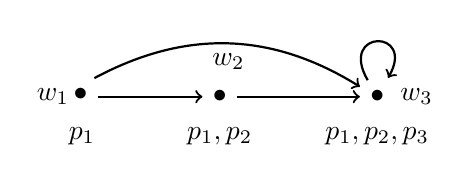
\begin{tikzpicture}[node distance=2cm, auto, thick]
      \node (w1) {$w_1 \, \bullet$} ; 
      \node (w2) [right of=w1]  {$\bullet$}; 
      \node (w3) [right of=w2] {$\bullet$} edge [in=60,out=120,loop] () ;
      \draw[->] (w1) to node {} (w2); \draw[->] (w2) to node {} (w3);
      \draw[->, bend left] (w1) to node [swap] {$w_2$} (w3); 
      \path node at ( 4.5,0) {$w_3$}; 
      \path node at ( 0.25,-0.5) {$p_1$}; 
      \path node at ( 2,-0.5) {$p_1,p_2$}; 
      \path node at ( 4,-0.5) {$p_1,p_2,p_3$};
      % \path node at ( 0,-1) [shape=circle,draw] {};
    \end{tikzpicture}
    %\node [circle,draw] {a} edge [in=30,out=60,loop] ();
  \end{center}
  Are the following !!{formula}s and schemas true in the model $\mModel{M}$,
  i.e., true at every world in $\mModel{M}$? Explain.
  \begin{enumerate}
  \item $p\lif \Diamond p$ (for $p$ atomic);
  \item $!A\lif \Diamond !A$ (for $!A$ arbitrary);
  \item $\Box p \lif p$ (for $p$ atomic);
  \item $\lnot p \lif \Diamond \Box p$ (for $p$ atomic);
  \item $\Diamond \Box !A$ (for $!A$ arbitrary);
  \item $\Box \Diamond p$ (for $p$ atomic). 
  \end{enumerate}
\end{prob}

\end{document}
